\documentclass{siproblemset}

\usepackage{multicol}
\usepackage{xcolor}
\usepackage{amsmath}

% SI Session Information
\course{MTH 1321}
\sessionnum{7}
\sessiondate{2/23/21}

\warmup{Overview of Basic Derivative Rules}
\topic{Evaluating Derivatives}
\cooldown{Applications of the Derivative}

% Worksheet Information
\title{Basic Derivative Rules}
\sections{Section 3.2}
\withnamespace

\begin{document}
    \maketitle
    
    \activity{Warmup}{Basic Derivative Rules}{Try these problems \textbf{alone} as your peers join the session. Do your best to not refer to your notes.}{15 minutes}
    
    \mcq[2]{Evaluate the following:}{
        \task $\dddx \left[ c\right] $
        \task $\dddx \left[ x^k\right] $
        \Tinysp
        \task $\dddx \left[cf(x)\right]$
        \task $\dddx \left[ f(x)\pm g(x)\right] $
        \Tinysp
        \task $\dddx \left[ e^x\right] $
        \task $\dddx \left[x\right]$
        \Tinysp
%        \task $\dddx \left[f(x)\cdot g(x)\right]$
        \task $\dddx \left[ \sqrt{x}\right] $
        \task $\dddx \left[ \dfrac1x\right] $
        \Tinysp
%        \task $\dddx \left[ \dfrac{f(x)}{g(x)}\right] $
    }
    \frq{What is the graphical relationship between a function and its derivative?}
    
    \pagebreak
    \activity{Activity 1}{Computing Derivatives Using Derivative Rules}{Work together in your \textbf{breakout rooms} to answer these questions. Do your best to not refer to your notes while working on these problems.}{30 minutes}

    \mcq{Compute the derivative.}{
        \task $f(x)=x^2(3+x^{-1})$
        \Normalsp
        \task $\dddx\left[ \left(\sqrt x - 1\right)\left(\sqrt x + 1\right)\right] $
        \Normalsp
        \task $\dddf{t}\left[t^{\sqrt{17}}\right]\Bigr|_{t=1}$
        \Normalsp
        \task $f(x)=9-12x^{1/3}+8e^x$
        \Normalsp
        \task $g(w)=(1+w)^3$
        \Largesp
        \task $h(t)=5e^{t-3}$
    }\pagebreak
    
    \activity{Activity 2}{Applications of the Derivative}{Work together in your \textbf{breakout rooms} to answer these questions. Do your best to not refer to your notes while working on these problems.}{30 minutes}
    
    \frq{Find the point(s) on the graph of the curve $y=\dfrac23x^3-5x-4$ at which the tangent line is parallel to $y=3x-2$}
    \Normalsp
    
    \frq{Draw the graph of $f'$ given the graph of $f$ below.}
    
    \begin{multicols}{2}
        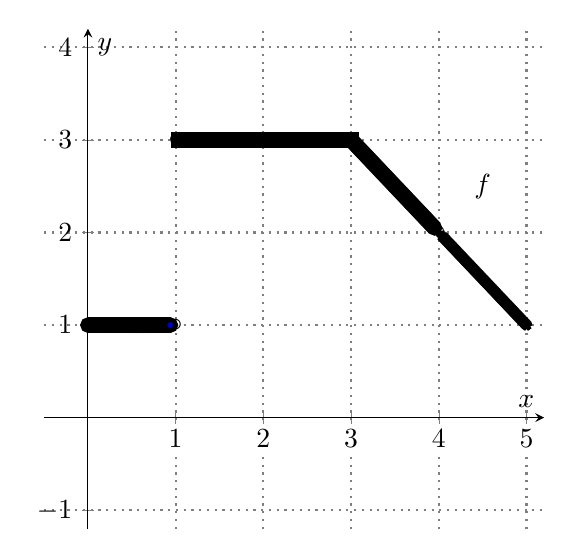
\begin{tikzpicture}
        \begin{axis}[axis x line=center, axis y line=middle,
        width=2.5in, height=2.5in, 
        scale only axis, %axis equal,
        xmin=-0.5, xmax=5.2,
        ymin=-1.2, ymax=4.2,
        xtick={0,...,5}, ytick={-1,...,4},
        xticklabel style={draw=none, inner sep=2pt, fill=white, text opacity=1},
        xlabel={$x$}, ylabel={$y$},
        grid=both, grid style={line width=.8pt, draw=gray, dotted},
        minor tick num=0, samples=100]
        \addplot+[black, ultra thick, domain=0:.94] {1};
        \addplot+[black, ultra thick, domain=1.03:3] {3};
        \addplot+[black, ultra thick, domain=3:3.95] {6-x};
        \addplot+[black, ultra thick, domain=4.04:5] {6-x};
        \node at (4.5,2.5) {$f$};
        \node at (1,1) {$\circ$};
        \node at (1,3) {$\circ$};
        \node at (4,2) {$\circ$};
        \node at (3,3) {$\bullet$};
        \end{axis}
        \end{tikzpicture}
        
        \columnbreak
        
        \begin{tikzpicture}
        \begin{axis}[axis x line=center, axis y line=middle,
        width=2.5in, height=2.5in, 
        scale only axis, %axis equal,
        xmin=-0.5, xmax=5.2,
        ymin=-4.2, ymax=1.2,
        xtick={0,...,5}, ytick={-4,...,1},
        xticklabel style={draw=none, inner sep=2pt, fill=white, text opacity=1},
        xlabel={$x$}, ylabel={$y$},
        grid=both, grid style={line width=.8pt, draw=gray, dotted},
        minor tick num=0]
        \end{axis}
        \end{tikzpicture}
    \end{multicols}
    \pagebreak
    \Tinysp
    \frq{Draw a possible graph of $g$ given the graph of $g'$ below.}
    
    \begin{multicols}{2}
        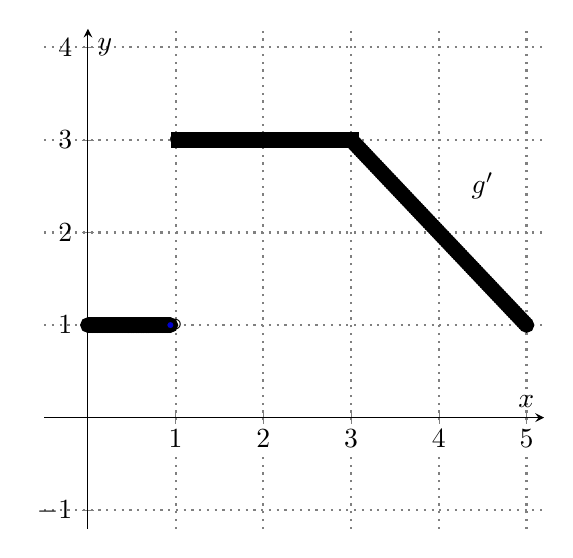
\begin{tikzpicture}
        \begin{axis}[axis x line=center, axis y line=middle,
        width=2.5in, height=2.5in, 
        scale only axis, %axis equal,
        xmin=-0.5, xmax=5.2,
        ymin=-1.2, ymax=4.2,
        xtick={0,...,5}, ytick={-1,...,4},
        xticklabel style={draw=none, inner sep=2pt, fill=white, text opacity=1},
        xlabel={$x$}, ylabel={$y$},
        grid=both, grid style={line width=.8pt, draw=gray, dotted},
        minor tick num=0, samples=100]
        \addplot+[black, ultra thick, domain=0:.94] {1};
        \addplot+[black, ultra thick, domain=1.03:3] {3};
        \addplot+[black, ultra thick, domain=3:5] {6-x};
        \node at (4.5,2.5) {$g'$};
        \node at (1,1) {$\circ$};
        \node at (1,3) {$\circ$};
        \node at (3,3) {$\bullet$};
        \end{axis}
        \end{tikzpicture}
        
        \columnbreak
        
        \begin{tikzpicture}
        \begin{axis}[axis x line=center, axis y line=middle,
        width=2.5in, height=2.5in, 
        scale only axis, %axis equal,
        xmin=-0.5, xmax=5.2,
        ymin=-2.4, ymax=8.4,
        xtick={0,...,5}, ytick={-2,0,...,8},
        xticklabel style={draw=none, inner sep=2pt, fill=white, text opacity=1},
        xlabel={$x$}, ylabel={$y$},
        grid=both, grid style={line width=.8pt, draw=gray, dotted},
        minor tick num=0]
        \end{axis}
        \end{tikzpicture}
    \end{multicols}
    \pagebreak

    \activity{Cooldown}{Properties of the Derivative}{Try these problems \textbf{alone}. Do your best to not refer to your notes.}{15 minutes}
    
    \mcq{State whether the following statements are always true (T) or always false (F). If the statement is conditionally true, explain.}{
        \task If $f(x)$ is continuous at $x=a$, then it is differentiable at $x=a$.
        \Tinysp
        \task If $f(x)$ is differentiable at $x=a$, then it is continuous at $x=a$.
        \Tinysp
        \task If $f(x)=x^2+3x^4$, then $f'(x)=2x+12x^3$.
        \Tinysp
        \task If $f'(x)=2x+12x^3$, then $f(x)=x^2+3x^4$.
        \Tinysp
        \task If $f'(2)=2$, then $f(x)$ is continuous at $x=2$.
        \Tinysp
        \task If $f(2)=2$, then $f'(2)$ exists.
        \Tinysp
        \task If $f(x)$ and $g(x)$ are not differentiable at $x=a$, then $h(x)=(f + g)(x)$ is not differentiable at $x=a$.
    }
\end{document}